
\section{Storage}\label{section:storage}

Storage component is used for storing internal platform data, acquired posts and analyses. This module provides an abstraction of physical databases for the rest of the components. Every other component can communicate with the internal part of the storage via REST API and all internal entities support a custom subset of CRUD operations. Posts and analyses can be stored via messaging, but they can be queried only via REST API. This approach should help to increase the performance of the whole platform and loose coupling between components.

\subsection{Requirements and Dependencies}

Storage module needs a relational database for storing internal platform data, but posts and analyses must be stored in a storage, where it is easier to query those data, so the second storage dependency is a search engine.

\begin{itemize}
    \item Run: Java\footnote{\url{https://www.java.com/en/}}
        \begin{itemize}
            \item Minimal version of Java: 11
            \item Minimal version of Maven: 3.3.9\footnote{\url{https://maven.apache.org}}
        \end{itemize}
    \item Relation database: PostgreSQL\footnote{\url{https://www.postgresql.org}}
        \begin{itemize}
            \item Recommended version of PostgreSQL: 9.6
        \end{itemize}
    \item Search engine: Elasticsearch\footnote{\url{www.elastic.co/elasticsearch}}
        \begin{itemize}
            \item Recommended version of Elasticsearch: 7.4.2
        \end{itemize}
    \item Kafka broker
        \begin{itemize}
            \item Platform component
        \end{itemize}
    \item Messaging
        \begin{itemize}
            \item Platform component
        \end{itemize}
\end{itemize}

\subsection{Code}

For implementation Java 11 language with Spring Boot framework\footnote{\url{https://spring.io}} is used. Spring Boot framework was chosen due to easier and faster development, because it is built on the Inversion of Control principle\footnote{\url{https://en.wikipedia.org/wiki/Inversionofcontrol}} and also it provides an abstraction of databases and other dependencies. For building of the whole application multi-module Maven is used.

During the design phase, we included MongoDB\footnote{\url{https://www.mongodb.com}} as NoSQL database for posts and analyses. After some time we have not found any reasonable real-world use case for duplication of data. (Synchronization performance was not great and the storage was using more physical disc space than needed.) Also, Elasticsearch has made internal improvements, so it is more often used as primary storage. 

User authentication and authorization is not implemented in the current version of Socneto, because it is beyond its primary scope. If there is some identity provider in the future, it will be simple to improve security with Spring Security\footnote{\url{https://spring.io/projects/spring-security}}. As a temporal solution, users are imported into the database during the start of the application. This solution should only simulate user authentication. The correct solution is more complex, because it has to be reused in many components of the whole platform.

Storage component is divided into four modules. Every module has a different usage: storage of internal data, storage of posts and analyses, Kafka consumer and REST controllers. The main pattern besides IOC is used MVC with more layers: controllers, validation on data transfer objects, domain layer, persistence.


\paragraph{Module internal-storage}

This module can be used for CRUD operations with internal data (components, jobs, users, etc.). For storing data PostgreSQL is used and communication are done via Spring framework. The framework adds an abstraction of storage for this module.

\begin{itemize}
    \item Major classes:
        \begin{itemize}
            \item \texttt{ComponentDto} - description of Analyzer or Acquirer component
            \item \texttt{ComponentDtoService} - operations for \texttt{ComponentDto}
            \item \texttt{ComponentJobConfigDto} - configuration of components for a single job
            \item \texttt{ComponentJobConfigDtoService} - operations for \texttt{ComponentJobConfigDto}
            \item \texttt{ComponentJobMetadataDto} - object, where every component can store its metadata for a single job
            \item \texttt{ComponentJobMetadataDtoService} - operations for \texttt{ComponentJobMetadataDto}
            \item \texttt{JobViewDto} - view configuration of a single job 
            \item \texttt{JobViewDtoService} - operations for \texttt{JobViewDto}
            \item \texttt{UserDto} - internal user and password
            \item \texttt{UserDtoService} - operations for UserDto
        \end{itemize}
    \item App properties config:
        \begin{itemize}
            \item \texttt{spring.datasource.url} - JDBC string to database
            \item \texttt{spring.datasource.username} - database user
            \item \texttt{spring.datasource.password} - database password
        \end{itemize}
    \item Spring concept:
        \begin{itemize}
            \item Spring Boot Starter JDBC
        \end{itemize}
    \item Dependencies:
        \begin{itemize}
            \item PostgreSQL database
        \end{itemize}
\end{itemize}

\subsubsection{Module analysis-results}

Module analysis-results uses Elasticsearch for storing posts and analyses. These objects can be queried in many ways:

Posts support search queries with pagination and aggregations by authors, language, etc.

\begin{description}
    \item Query \texttt{POST\_AGGREGATION}:
    \begin{itemize}
        \item \texttt{COUNT\_PER\_TIME} - aggregation of posts over time
        \item \texttt{COUNT\_PER\_AUTHOR} - aggregation of posts per authors
        \item \texttt{COUNT\_PER\_LANGUAGE} - aggregation of posts per languages
    \end{itemize}
\end{description}

Analyses can be queried in a more complex way. The basic list with results can be queried with pagination, but also aggregation over list and map results is supported.

\begin{description}
    \item Query \texttt{AGGREGATION}:
    \begin{itemize}
        \item \texttt{MAP\_SUM} - sums occurences in \texttt{MapValue} result
        \item \texttt{LIST\_COUNT} - sums occurences in \texttt{ListValue} result
    \end{itemize}
    \item Query \texttt{LIST}:
    \begin{itemize}
        \item \texttt{LIST} - list of analyset result values
        \item \texttt{LIST\_WITH\_TIME} - list of analyset result values with time
    \end{itemize}
\end{description}

\begin{itemize}
    \item Major classes:
        \begin{itemize}
            \item \texttt{SearchPostDto} - an acquired post entity
            \item \texttt{SearchPostDtoService} - operations for SearchAnalysisDtoService
            \item \texttt{SearchAnalysisDto} - an analysis entity 
            \item \texttt{SearchAnalysisResultDto} - representation of analysis result value
            \item \texttt{SearchAnalysisDtoService} - operations for SearchAnalysisDtoService
            \item \texttt{ResultRequest} - a request for list values or agrregations
            \item \texttt{ResultService} - an aggregation service for posts and analyses
            \item \texttt{ListWithCount} - a result of list request with a total count filed
        \end{itemize}
    \item App properties config:
        \begin{itemize}
            \item \texttt{elasticsearch.host} - Elasticsearch host
            \item \texttt{elasticsearch.port} - Elasticsearch port
        \end{itemize}
    \item Spring concept:
        \begin{itemize}
            \item Spring Data Elasticsearch
        \end{itemize}
    \item Dependencies:
        \begin{itemize}
            \item Elasticsearch
        \end{itemize}
\end{itemize}

\subsubsection{Module storage-messaging}

This module is created for receiving posts and analysis messages from the Kafka message broker. Every message is parsed into an internal object and stored by the analysis-results module. The module consists of two configurable receivers for different topics.

\begin{itemize}
    \item Major classes:
        \begin{itemize}
            \item \texttt{AnalysisReceiver} - a consumer of analyses messages
            \item \texttt{PostReceiver} - a consumer of posts messages
            \item \texttt{KafkaConsumerConfig} - a consumer factory provider
        \end{itemize}
    \item App properties config:
        \begin{itemize}
            \item \texttt{spring.messaging.bootstrap-servers} - url to Kafka server
            \item \texttt{app.topic.toDbRaw} - a topic for post messages
            \item \texttt{app.topic.toDbAnalyzed} - a topic for analysis messages
        \end{itemize}
    \item Spring concept:
        \begin{itemize}
            \item Spring Kafka 
        \end{itemize}
    \item Dependencies:
        \begin{itemize}
            \item \texttt{analysis-results} module
            \item Kafka message broker
        \end{itemize}
\end{itemize}

\subsubsection{Module storage-web}

Storage-web module contains all REST endpoints of the storage component. It uses CRUD services from Internal-storage module and search services from Analysis-storage module.

Also, this module is the only one which can be run. For execution Spring Boot Starter is used, which starts all modules together, loads configuration, connects to Kafka, database, etc.

Validation of input API objects is done via \texttt{javax.*} annotations. This approach helps with validation without a huge amount of code and it is built on Spring framework.

\begin{itemize}
    \item Major classes:
        \begin{itemize}
            \item \texttt{ComponentController} - REST API for components
            \item \texttt{ComponentJobConfigController} - REST API for component job configs
            \item \texttt{ComponentJobMetadataController} - REST API for component job metadata
            \item \texttt{HealthCheckController} - health check endpoint
            \item \texttt{JobController} - REST API for jobs
            \item \texttt{JobViewController} - REST API for job view
            \item \texttt{PostController} - REST API for posts
            \item \texttt{ResultsController} - REST API for results
            \item \texttt{UserController} - REST API for users
        \end{itemize}
    \item App properties config:
        \begin{itemize}
            \item \texttt{app.componentId} - ID of Storage component
            \item \texttt{server.port} - Port of Storage component
        \end{itemize}
    \item Spring concept:
        \begin{itemize}
            \item Spring Boot Starter Web
        \end{itemize}
    \item Dependencies:
        \begin{itemize}
            \item \texttt{internal-storage}
            \item \texttt{analysis-results}
        \end{itemize}
\end{itemize}

\subsection{Build + Run}

\begin{itemize}
    \item Build: \texttt{maven package -f pom.xml}
    \item Run: \texttt{java -jar storage-web-1.0.0-SNAPSHOT.jar}
\end{itemize}

\subsection{Communication}\label{subsection:storage-communication}

The storage component provides two APIs. Kafka API is only for acquired posts and analyses. This API provides async communication for acquirers and analysers. For querying posts and analyses the REST API must be used. Both endpoints support pagination when it is needed. REST API is also used for CRUD operations of internal data. For better understanding, the flow is described in Diagram \ref{figure:storage}.

\begin{figure}[H]
\centering
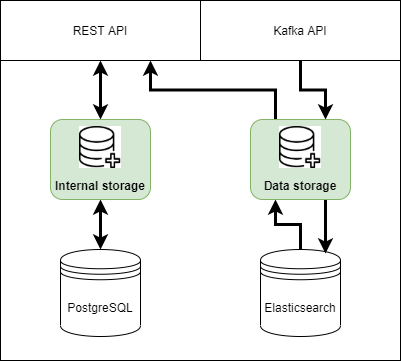
\includegraphics[width=8cm]{diagrams/socneto-storage.png}
\caption{Storage architecture uses two databases forming polyglot storage}
\label{figure:storage}
\end{figure}

\begin{itemize}
    \item REST
        \begin{itemize}
            \item Swagger: \texttt{$<$storage-host$>$:$<$storage-port$>$/swagger-ui.html}
            \item Exported swagger documentation: \texttt{docs/api/storage-api.pdf}
        \end{itemize}
    \item Messaging topics
        \begin{itemize}
            \item Posts:
            \texttt{job\_management.component\_data\_input.storage\_db}
            \item Analyses:
            \texttt{job\_management.component\_data\_analyzed\_input.storage\_db}
        \end{itemize}
\end{itemize}
